\noindent Jazykové technológie sú informačné technológie, ktoré
sa zameriavajú na prácu s~ľudským jazykom, preto sa tieto
technológie často zaraďujú pod pojem ľudské jazykové
technológie. Ľudský jazyk existuje v~hovorenej a~písomnej forme.
Kým reč je najstarší a~najprirodzenejší spôsob jazykovej
komunikácie, komplexné informácie a~súhrn ľudského poznania sa
zaznamenávajú a~prenášajú vo forme písomných textov. Rečové
a~textové technológie spracúvajú alebo produkujú jazyk v~uvedených
dvoch formách. Ale jazyk má tiež aspekty spoločné pre obe formy,
ako sú slovníky, väčšina z~gramatiky a~zmysel viet. Veľkú časť
jazykových technológií teda nemožno zaradiť výlučne pod rečovú
alebo textovú technológiu. Znalostné technológie sú technológie,
ktoré spájajú jazyk s~vedomosťami. Obrázok \ref{fig:ltincontextsk}
znázorňuje záber jazykových technológií. V~našej komunikácii
miešame jazyk s~inými druhmi komunikácie a~ďalšími informačnými
médiami. Reč kombinujeme s~gestami a~výrazmi tváre. Texty je možné
kombinovať s~obrázkami a~zvukmi. Filmy môžu obsahovať jazyk
v~hovorenej aj písomnej forme. Rečové a~textové technológie sa teda
prekrývajú a~pôsobia v~interakcii s~mnohými ďalšími
technológiami, ktoré uľahčujú spracovanie multimodálnej
komunikácie a~multimediálnych dokumentov.

\begin{figure*}[ht]
  \colorrule{grey3}{\textwidth}{1.5pt}
  \center
  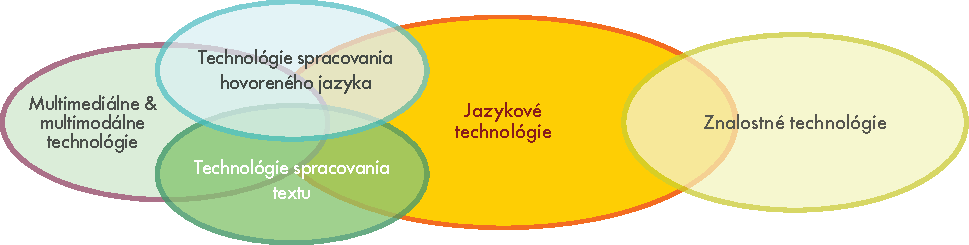
\includegraphics[width=\textwidth]{../_media/slovak/language_technologies}
  \caption{Záber jazykových technológií}
  \label{fig:ltincontextsk}
  \colorrule{grey3}{\textwidth}{1.5pt}
\end{figure*}

